\documentclass[a4paper, 12pt, final, garamond]{book}
\usepackage{cours-preambule}

\raggedbottom

\makeatletter
\renewcommand{\@chapapp}{Optique -- chapitre}
\makeatother

\begin{document}
\setcounter{chapter}{1}

\chapter{TD~: Base de l'optique g\'eom\'etrique}

\section{Fréquence, longueur d'onde et indice}
La lumière visible possède des longueurs d'onde dans le vide comprises entre
\SIrange{400}{800}{nm}.
\begin{enumerate}
    \item À quel intervalle de fréquences cela correspond-il~?
    \item Que deviennent ces longueurs d'ondes
        \begin{enumerate}
            \item dans l'eau d'indice $n_1 = \num{1.33}$~?
            \item dans un verre d'indice $n_2 = \num{1.5}$~?
        \end{enumerate}
    \item Calculer la valeur de la vitesse de la lumière dans un verre d'indice
        $n = \num{1.5}$.
\end{enumerate}

\section{Détermination directe de l'indice d'un liquide}
\begin{wrapfigure}[4]{R}{.3\linewidth}
    \vspace*{-1.5cm}
    \centering
    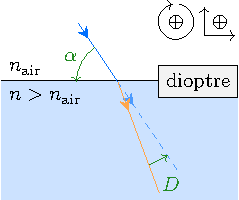
\includegraphics[width=\linewidth]{dioptre_alpha-horiz_plain}
    \label{fig:alpha_horiz}
\end{wrapfigure}
\vspace{1cm}
Un rayon lumineux dans l'air ($n_{\rm air}$) tombe sur la surface horizontale
d'un liquide d'indice $n$. Il fait un angle $\alpha = \ang{56;;}$ avec le plan
horizontal. La déviation entre le rayon incident et le rayon réfracté est
$\theta = \ang{13.5;;}$. Quel est l'indice $n$ du liquide~?
\vspace{1cm}

\section{Détecteur de pluie sur un pare-brise}
\begin{wrapfigure}[8]{R}{.3\linewidth}
    \vspace*{10pt}
    \centering
    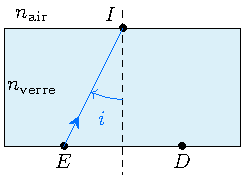
\includegraphics[width=\linewidth]{pluie_plain.pdf}
    \label{fig:pluie_plain}
\end{wrapfigure}
On modélise un pare-brise par une lame de verre à faces parallèles, d'épaisseur
$e = \SI{5.00}{mm}$, d'indice $n_v = \num{1.5}$. Un fin pinceau lumineux issu d'un
émetteur situé en $E$ arrive de l'intérieur du verre sur le dioptre verre
$\rightarrow$ air en $I$ avec un angle d'incidence $i = \ang{60.;;}$.
\begin{enumerate}
    \item Montrer que le flux lumineux revient intégralement sur le détecteur
        situé en $D$ et déterminer la distance $ED$.
    \item Lorsqu'il pleut, une lame d'eau d'indice $n_e = \num{1.33}$ et
        d'épaisseur $e' = \SI{1.00}{mm}$ se dépose sur un pare-brise. Représenter
        le rayon lumineux dans ce cas. À quelle distance du détecteur
        arrive-t-il~?
\end{enumerate}

\section{Rayon lumineux à travers une vitre}
Un rayon lumineux traverse une vitre d'épaisseur $a = \SI{5.0}{mm}$ et d'indice
$n = \num{1.5}$ sous une incidence $i_1 = \ang{45;;}$. Le milieu extérieur est
l'air.

\begin{enumerate}
    \item Faire un schéma et calculer l'angle de réfraction $i_2$ lors du
        passage à travers la première face (air$\rightarrow$verre).
    \item Calculer l'angle de réfraction $i_3$ lors du passage à travers la
        deuxième face (verre$\rightarrow$air).
    \item Montrer que le rayon entrant et le rayon sortant sont parallèles.
    \item Calculer la déviation latérale $d$ (la distance entre le point où sort
        le rayon émergeant et celui où sortirait le rayon incident s'il n'était
        pas dévié) entre ces deux rayons.
\end{enumerate}

\section{Fibre optique à saut d'indice}

Les câbles à fibres optiques permettent la transmission à haut débit de tous
types de signaux électromagnétiques, sur de longues distances avec très peu
d'atténuation~; ceux-ci se propagent comme la lumière. Chaque câble comporte un
grand nombre de fibres très fines.

Une fibre optique à saut d'indice peut être assimilée à un cylindre de
révolution d'axe $Oz$, constitué d'un cœur de rayon $a$ (de l'ordre de 8 à
\SI{50}{\micro m}) et d'indice $n_1$, entouré d'une couche cylindrinque appelée
\textit{gaine}, d'épaisseur $b-a$ et d'indice $n_2 < n_1$.

\begin{figure}[h]
    \centering
    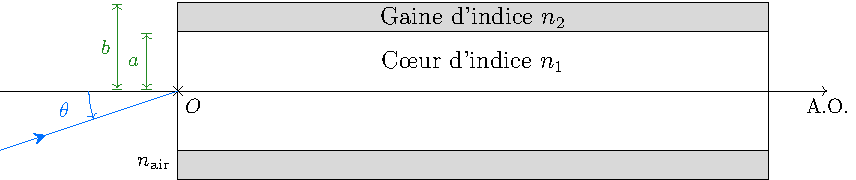
\includegraphics[width=.8\linewidth]{fibre_plain.pdf}
    \captionsetup{justification=centering}
    \caption{Schéma d'une fibre optique à saut d'indice.}
    \label{fig:fibre_plain}
\end{figure}

Un rayon pénètre depuis l'air dans la fibre par sa base en $O$, en faisant un
angle $\theta$ avec l'axe optique confondu avec $Oz$. Exprimer une condition sur
$\theta$ en fonction des indices $n_1$ et $n_2$ pour que le rayon se propage
uniquement dans le cœur de la fibre.

\section{Mirages}

Cet exercice est une introduction à la propagation de la lumière dans un milieu
non homogène. Le but est d'interpréter qualitativement les phénomènes de mirages
(froid et chaud). Ces illusions d'optiques apparaissent lorsque l'indice de
l'air varie assez rapidement avec l'altitude.
\begin{enumerate}
    \item Lorsque le sol est très «~chaud~», la température de l'air est
        d'autant plus élevée qu'il est proche du sol. Plus la température de
        l'air est élevée, moins son indice optique est élevé. On décompose
        l'atmosphère en N couches planes isothermes dont l'indice optique
        augmente avec l'altitude~:
        \[ \forall k \in \Nb^* \quad\text{et}\quad 1 \leq k \leq N,
        \quad n_{k+1} > n_k\]
        \begin{minipage}{0.47\linewidth}
            \begin{center}
                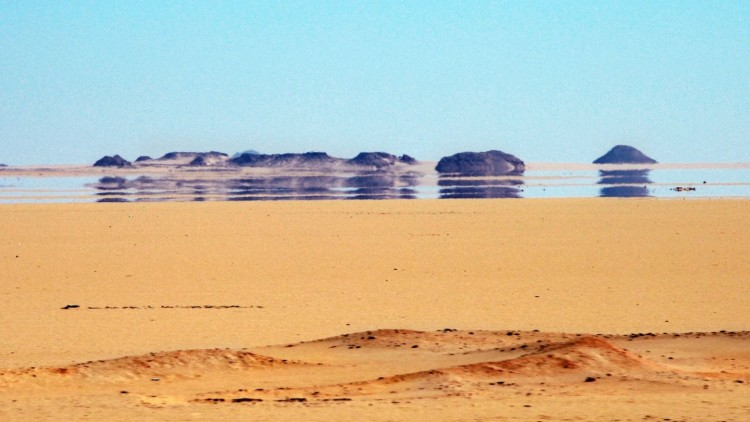
\includegraphics[width=\linewidth]{mirage_chaud}
                \captionof{figure}{Photo d'un mirage chaud}
                \label{fig:mir_chaud}
            \end{center}
        \end{minipage}
        \hfill
        \begin{minipage}{0.47\linewidth}
            \begin{center}
                \centering
                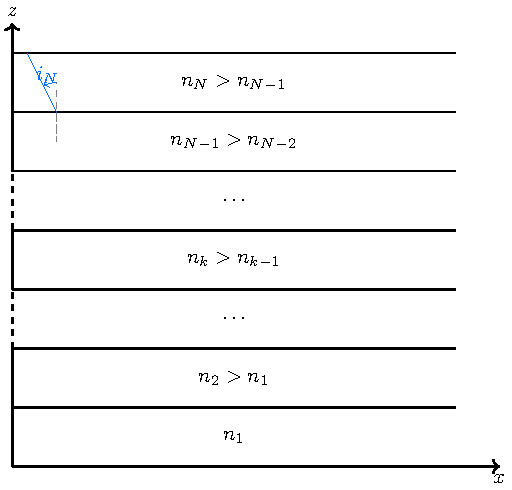
\includegraphics[height=5cm]{mirage_plain.pdf}
                \captionof{figure}{Modèle d'atmosphère stratifié}
                \label{fig:mirage_plain}
            \end{center}
        \end{minipage}
    \begin{enumerate}
        \item Montrer que $n_k\sin(i_k)$ est constant, où $k$ désigne la
            $k$-ième couche atmosphérique.
        \item Tracer les rayons réfractés par les couches d'air successives en
            faisant apparaître les angles d'incidence et de réfraction, puis
            montrer que pour un angle d'incidence initial suffisamment grand,
            une réflexion totale se produit.
        \item Pour une variation continue de l'indice $n$, tracer
            qualitativement le trajet d'un rayon lumineux issu du ciel. Dans
            quel sens et direction sa trajectoire est-elle courbée~?
        \item Interpréter alors le mirage chaud observé sur la photo ci-dessus.
            Faire un schéma.
    \end{enumerate}

    \item Il arrive que la mer soit nettement plus «~froide~» que l'atmosphère.
        La température de l'air augmente alors avec l'altitude. Que peut-on
        observer si on regarde un bateau ou une île au loin~? Interpréter le
        mirage froid de la photo page suivante. Justifier par un schéma.
        \begin{figure}[h]
            \centering
            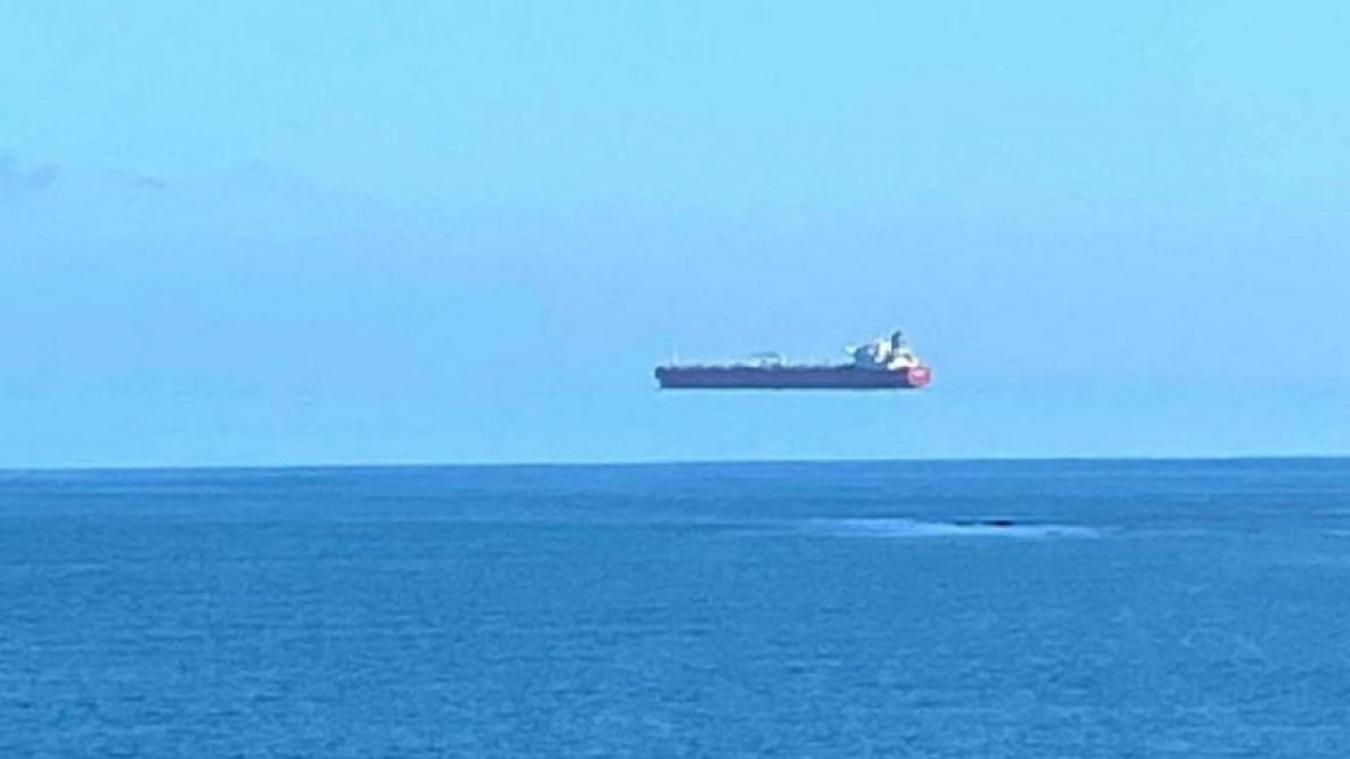
\includegraphics[width=.5\linewidth]{mirage_froid}
            \captionsetup{justification=centering}
            \caption{Photo d'un mirage froid}
            \label{fig:mir_froid}
        \end{figure}
\end{enumerate}

\section{Réfractomètre de Pulrich}
\begin{wrapfigure}[6]{R}{.3\linewidth}
    \vspace*{-20pt}
    \centering
    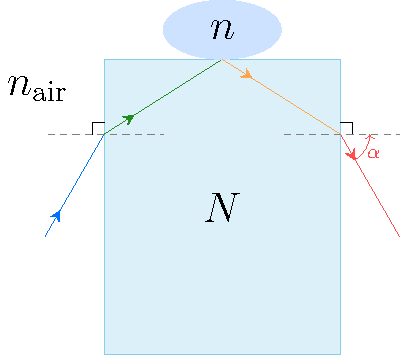
\includegraphics[width=\linewidth]{pulrich_plain}
    \label{fig:pulrich_plain}
\end{wrapfigure}

Un réfractomètre de Pulrich est constitué d'un bloc de verre de section
rectangulaire d'indice $N$ connu, sur lequel on a déposé une goutte de liquide
d'indice $n$ inconnu ($n < N$). On observe un faisceau de rayons parallèles à la
limite réfraction/réflexion totale et on mesure en sortie l'angle $\alpha$ dans
ce cas.
\begin{enumerate}
    \item Établir l'expression de $n$ en fonction de $N$ et $\alpha$.
    \item Application numérique~: calculer $n$ sachant que $N = \num{1.626}$ et
        $\alpha = \ang{60;00;}$.
\end{enumerate}

\section{Incidence de Brewster}
Un dioptre plan séparer l'air d'un milieu d'indice $n$. Pour quelle valeur de
l'angle d'incidence le rayon réfléchi est-il perpendiculaire au rayon réfracté~?

\section{Réfraction et dispersion}
Un rayon lumineux, se propageant dans l'air, arrive avec une incidence $i =
\ang{40;;}$
sur un dioptre air/verre plan. Si on considère que ce rayon est constitué de
lumière blanche, calculer l'écart angulaire entre les rayons réfractés extrêmes.

\textit{Données}~: l'indice du verre est donné par la formule de Cauchy~: $\DS n
= A + \frac{B}{\lambda_0{}^2}$, avec $A = \num{1.504}$ et $B =
\SI{4.188e-15}{m^2}$~; l'indice de l'air est $n_{\rm air} = \num{1.000}$.

\end{document}
